\documentclass{article}
\usepackage[utf8]{inputenc}
\usepackage{amsmath}
\usepackage{amssymb}
\usepackage{circuitikz}
\usepackage[makeroom]{cancel}
\usepackage{graphicx}

\setlength{\parskip}{1em}
\renewcommand{\arraystretch}{2}

\title{Homework 1}
\date{2021 January 26}
\author{John J Li}

\begin{document}
    \pagenumbering{gobble}
    \maketitle
    \noindent
    Please excuse this atrocious attempt at LaTex. I have just begun learning
    and I am still unfamiliar with some of the scripts.

    \noindent
    But after 800+ lines of code and many hours, I have decided that perhaps my way of writing LaTex is not the most effecient
    method to do homework.
    \newpage
    \pagenumbering{arabic}

    \noindent
    Here are the answers to the problems. The subsequent work are located further in
    the document.

    \textbf{Problem 1:}

    \quad \textbf{a)}

    \quad\quad $2^{13} + 2^{12} + 2^9 + 2^6 + 2^4 + 2^2 + 2 = \boxed{12886}$

    \quad \textbf{b)} 0001011110

    \quad\quad $2^6 + 2^4 + 2^3 + 2^2 + 2^1 = \boxed{94}$

    \quad \textbf{c)} 101010110010

    \quad\quad $2^{11} + 2^9 + 2^7 + 2^5 + 2^4 + 2 = \boxed{2738}$

    \textbf{Problem 2:}

    \quad \textbf{a)} 823

    \quad\quad 823 in binary is \boxed{001100110111_2}

    \quad \textbf{b)} 209

    \quad\quad 209 in binary is \boxed{000011010001_2}

    \textbf{Problem 3:}

    \quad \textbf{a)} $1011000101000010111_2$

    \quad\quad \boxed{58A17_{16}}

    \quad \textbf{b)} $1938_{10}$

    \quad\quad \boxed{7C2_{16}}

    \textbf{Problem 4:}

    \quad \textbf{a)} 2FACED

    \quad\quad $2 \times 16^5 + 
        15 \times 16^4 + 
        10 \times 16^3 +
        12 \times 16^2 + 
        14 \times 16^1 + 
        13 \times 16^0 = \boxed{3124461}$

    \textbf{Problem 5:}
    
    $G = B(C+A) \oplus ((A'B) + (B+C)')$
    \begin{center}
        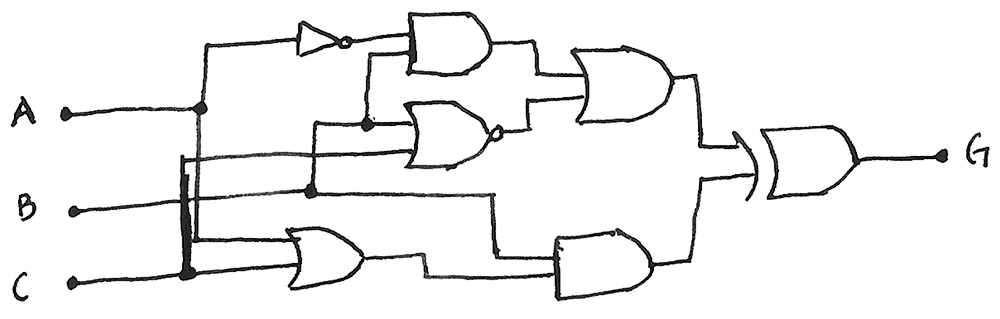
\includegraphics{001.png}
    \end{center}

    \quad\quad
    \noindent\fbox{%
        \parbox{\textwidth}{%
            If ABC = 110, respectively, G would equal 1
        }%
    }

    \textbf{Problem 6:}

    \quad\quad
    \noindent\fbox{%
        \parbox{\textwidth}{%
            The two functions are not equal
        }%
    }

    \textbf{Problem 7:}

    \quad\quad
    \noindent\fbox{%
        \parbox{\textwidth}{%
            a can be either 0 or 1, but b has to be the opposite of a. For example,
            if a is 0 then b is 1 or vice versa.
        }%
    }

    \textbf{Problem 8:}

    \quad \textbf{a)} $101101+010101$

    \begin{center}
        \begin{tabular}{ ccccccc }
            & $1^1$ & $0^1$ & $1^1$ & 1 & $0^1$ & 1 \\
            + & 0   & 1   & 0   & 1 & 0   & 1 \\
            \hline
            overflow & 0 & 0 & 0 & 0 & 1 & 0
        \end{tabular}
        \quad\quad 
        \begin{tabular}{ ccc }
            & 4 & 5 \\
            + & 2 & 1 \\
            \hline
            overflow & & 2
        \end{tabular}
    \end{center}

    \quad \textbf{b)} $000101 + 010010$

    \begin{center}
        \begin{tabular}{ ccccccc }
              & 0 & 0 & 0 & 1 & 0 & 1 \\
            + & 0 & 1 & 0 & 0 & 1 & 0 \\
            \hline
            & 0 & 1 & 0 & 1 & 1 & 1
        \end{tabular}
        \quad\quad 
        \begin{tabular}{ ccc }
            & & 5 \\
            + & 1 & 8 \\
            \hline
            & 2 & 3
        \end{tabular}
    \end{center}

    \textbf{Problem 9:}

    \quad \textbf{a)} +20

    \quad\quad \boxed{010100}

    \quad \textbf{b)} -30

    \quad\quad \boxed{100010}

    \textbf{Problem 10:}

    \quad \textbf{a)} 110000

    \quad\quad \boxed{-16}

    \quad \textbf{b)} 011010

    \quad\quad \boxed{+26}

    \textbf{Problem 11:}

    \quad \textbf{a)} 7 + 18

    \begin{center}
        \begin{tabular}{ ccccccc }
              & 0 & 0 & $0^1$ & $1^1$ & 1 & 1 \\
            + & 0 & 1 & 0 & 0 & 1 & 0  \\
            \hline
            & 0 & 1 & 1 & 0 & 0 & 1
        \end{tabular}
        \quad\quad 
        \begin{tabular}{ ccc }
            & & 7 \\
            + & 1 & 8 \\
            \hline
            & 2 & 5
        \end{tabular}
    \end{center}

    \quad \textbf{b)} 12-29

    \begin{center}
        \begin{tabular}{ ccccccc }
              & 0 & 0 & 1 & 1 & 0 & 0 \\
            + & 1 & 0 & 0 & 0 & 1 & 1  \\
            \hline
            & 1 & 0 & 1 & 1 & 1 & 1
        \end{tabular}
        \quad\quad 
        \begin{tabular}{ ccc }
            & 1 & 2 \\
            - & 2 & 9 \\
            \hline
            -& 1 & 7
        \end{tabular}
    \end{center}

    \textbf{Problem 12:}

    \begin{center}
        \begin{tabular}{ c|c|c|c|c }
            A & B & C & D & F \\
            \hline
            0 & 0 & 0 & 0 & 1 \\
            0 & 0 & 0 & 1 & 1 \\
            0 & 0 & 1 & 0 & 1 \\
            0 & 0 & 1 & 1 & 1 \\
            0 & 1 & 0 & 0 & 1 \\
            0 & 1 & 0 & 1 & 1 \\
            0 & 1 & 1 & 0 & 1 \\
            0 & 1 & 1 & 1 & 0 \\
            1 & 0 & 0 & 0 & 1 \\
            1 & 0 & 0 & 1 & 0 \\
            1 & 0 & 1 & 0 & 1 \\
            1 & 0 & 1 & 1 & 0 \\
            1 & 1 & 0 & 0 & 1 \\
            1 & 1 & 0 & 1 & 0 \\
            1 & 1 & 1 & 0 & 0 \\
            1 & 1 & 1 & 1 & 1
            
        \end{tabular}
    \end{center}

    \textbf{Problem 13:}

    \quad\textbf{a)} 2 great gross + 7 gross + 4 dozen + 10 cans

    \quad\quad $2\times 12^3 + 7 \times 12^2 + 4 \times 12^1 + 10 \times 12^0=\boxed{4522}$

    \quad\textbf{b)} $6903_{10}$

    \quad\quad
    \noindent\fbox{%
        \parbox{\textwidth}{%
            3 great gross + 11 gross + 11 dozen + 10 cans
        }%
    }

    \textbf{Problem 14:}

    \quad\quad 2021 in hex is \boxed{7E5_{16}}

    \textbf{Problem 15:}



    \textbf{Problem 16:}

    \quad\textbf{a)} $-23 - 13$

    \begin{center}
        \begin{tabular}{ ccccccc }
              & 1 & 0 & 1 & 0 & 0 & 1 \\
            + & 1 & 1 & 0 & 0 & 1 & 1  \\
            \hline
            overflow & 0 & 1 & 1 & 1 & 0 & 0
        \end{tabular}
        \quad\quad 
        \begin{tabular}{ ccc }
            - & 2 & 3 \\
            - & 1 & 3 \\
            \hline
            overflow & 2 & 6
        \end{tabular}
    \end{center}

    \newpage
    \textbf{Problem 1:}

    \quad \textbf{a)} 11001001010110

    \begin{center}
        \begin{tabular}{ c|c|c|c|c|c|c|c|c|c|c|c|c|c }
            1 & 1 & 0 & 0 & 1 & 0 & 0 & 1 & 0 & 1 & 0 & 1 & 1 & 0 \\
            \hline
            $2^{13}$ & $2^{12}$ & 0 & 0 & $2^9$ & 0 & 0 & $2^6$ & 0 & $2^4$ & 0 & $2^2$ & $2^1$ & 0
        \end{tabular}
    \end{center}

    \quad\quad $2^{13} + 2^{12} + 2^9 + 2^6 + 2^4 + 2^2 + 2 = \boxed{12886}$

    \quad \textbf{b)} 0001011110

    \begin{center}
        \begin{tabular}{ c|c|c|c|c|c|c|c|c|c }
            0 & 0 & 0 & 1 & 0 & 1 & 1 & 1 & 1 & 0 \\
            \hline
            0 & 0 & 0 & $2^6$ & 0 & $2^4$ & $2^3$ & $2^2$ & $2^1$ & 0
        \end{tabular}
    \end{center}

    \quad\quad $2^6 + 2^4 + 2^3 + 2^2 + 2^1 = \boxed{94}$

    \quad \textbf{c)} 101010110010

    \begin{center}
        \begin{tabular}{ c|c|c|c|c|c|c|c|c|c|c|c }
            1 & 0 & 1 & 0 & 1 & 0 & 1 & 1 & 0 & 0 & 1 & 0\\
            \hline
            $2^{11}$ & 0 & $2^9$ & 0 & $2^7$ & 0 & $2^5$ & $2^4$ & 0 & 0 & $2^1$ & 0
        \end{tabular}
    \end{center}

    \quad\quad $2^{11} + 2^9 + 2^7 + 2^5 + 2^4 + 2 = \boxed{2738}$

    \textbf{Problem 2:}

    \quad \textbf{a)} 823

    \begin{center}
        \begin{tabular}{ c|c c }
            Bit 0 & $\frac{823}{2} = (2)411 + 1 \Rightarrow$ & 1 \\
            Bit 1 & $\frac{411}{2} = (2)205 + 1 \Rightarrow$ & 1 \\
            Bit 2 & $\frac{205}{2} = (2)102 + 1 \Rightarrow$ & 1 \\
            Bit 3 & $\frac{102}{2} = (2)51 + 0 \Rightarrow$ & 0 \\
            Bit 4 & $\frac{51}{2} = (2)25 + 1 \Rightarrow$ & 1 \\
            Bit 5 & $\frac{25}{2} = (2)12 + 1 \Rightarrow$ & 1 \\
            Bit 6 & $\frac{12}{2} = (2)6 + 0 \Rightarrow$ & 0 \\
            Bit 7 & $\frac{6}{2} = (2)3 + 0 \Rightarrow$ & 0 \\
            Bit 8 & $\frac{3}{2} = (2)1 + 1 \Rightarrow$ & 1 \\
            Bit 9 & $\frac{1}{2} = (2)0 + 1 \Rightarrow$ & 1 \\
            Bit 10 & $\frac{0}{2} = (2)0 + 0 \Rightarrow$ & 0 \\
            Bit 11 & $\frac{0}{2} = (2)0 + 0 \Rightarrow$ & 0
        \end{tabular}
    \end{center}

    \quad\quad 823 in binary is \boxed{001100110111_2}

    \quad \textbf{b)} 209

    \begin{center}
        \begin{tabular}{ c|c c }
            Bit 0 & $\frac{209}{2} = (2)104 + 1 \Rightarrow$ & 1 \\
            Bit 1 & $\frac{104}{2} = (2)52 + 0 \Rightarrow$ & 0 \\
            Bit 2 & $\frac{52}{2} = (2)26 + 0 \Rightarrow$ & 0 \\
            Bit 3 & $\frac{26}{2} = (2)13 + 0 \Rightarrow$ & 0 \\
            Bit 4 & $\frac{13}{2} = (2)6 + 1 \Rightarrow$ & 1 \\
            Bit 5 & $\frac{6}{2} = (2)3 + 0 \Rightarrow$ & 0 \\
            Bit 6 & $\frac{3}{2} = (2)1 + 1 \Rightarrow$ & 1 \\
            Bit 7 & $\frac{1}{2} = (2)0 + 1 \Rightarrow$ & 1 \\
            Bit 8 & $\frac{0}{2} = (2)0 + 0 \Rightarrow$ & 0 \\
            Bit 9 & $\frac{0}{2} = (2)0 + 0 \Rightarrow$ & 0 \\
            Bit 10 & $\frac{0}{2} = (2)0 + 0 \Rightarrow$ & 0 \\
            Bit 11 & $\frac{0}{2} = (2)0 + 0 \Rightarrow$ & 0
        \end{tabular}
    \end{center}

    \quad\quad 209 in binary is \boxed{000011010001_2}

    \textbf{Problem 3:}

    \quad \textbf{a)} $1011000101000010111_2$

    \quad\quad $0101 \; 1000 \; 1010 \; 0001 \; 0111 \Rightarrow$
    
    \begin{center}
        \begin{tabular}{ c|c }
            0111 & 7 \\
            0001 & 1 \\
            1010 & A \\
            1000 & 8 \\
            0101 & 5
        \end{tabular}
    \end{center}

    \quad\quad \boxed{58A17_{16}}

    \quad \textbf{b)} $1938_{10}$

    \begin{center}
        \begin{tabular}{ c|c c }
            Bit 0 & $\frac{1938}{16} = (16)124 + 2 \Rightarrow$ & 2 \\
            Bit 1 & $\frac{124}{16} = (16)7 + 12 \Rightarrow$ & $12 \Rightarrow C$ \\
            Bit 2 & $\frac{7}{16} = (16)0 + 7 \Rightarrow$ & 7
        \end{tabular}
    \end{center}

    \quad\quad \boxed{7C2_{16}}

    \textbf{Problem 4:}

    \quad \textbf{a)} 2FACED

    \begin{center}
        $2 \Rightarrow  2 \times 16^5$ \\
        $F \Rightarrow 15 \times 16^4$ \\
        $A \Rightarrow 10 \times 16^3$ \\
        $C \Rightarrow 12 \times 16^2$ \\
        $E \Rightarrow 14 \times 16^1$ \\
        $D \Rightarrow 13 \times 16^0$ \\
    \end{center}

    \quad\quad $2 \times 16^5 + 
        15 \times 16^4 + 
        10 \times 16^3 +
        12 \times 16^2 + 
        14 \times 16^1 + 
        13 \times 16^0 = \boxed{3124461}$

    \textbf{Problem 5:}
    
    $G = B(C+A) \oplus ((A'B) + (B+C)')$
    \begin{center}
        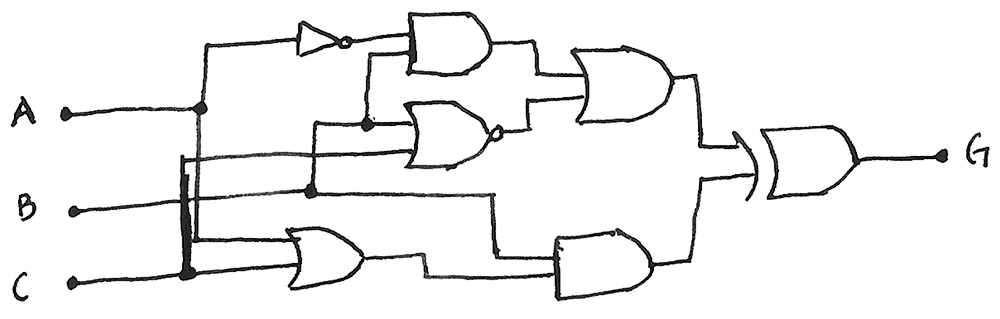
\includegraphics{001.png}
    \end{center}

    \quad\quad
    \noindent\fbox{%
        \parbox{\textwidth}{%
            If ABC = 110, respectively, G would equal 1
        }%
    }

    % \begin{circuitikz} 
    %     \draw
    %         (0,0) node [not port] (notA) {}
    %         (notA.in 1) node [] (A1) {A}
    %         (4,0) node [and port] (andAB) {}
    %         (andAB.in 2) node [anchor=east,xshift=-1cm] (B1) {B}
    %         (0,2) node [or port] (orBC) {}
    %     ;

    %     \draw (notA.out) -- (andAB.in 1);

    % \end{circuitikz}

    \textbf{Problem 6:}

    \quad\quad
    \noindent\fbox{%
        \parbox{\textwidth}{%
            The two functions are not equal
        }%
    }

    \begin{center}
        \begin{tabular}{ c|c|c|c|c|c|c|c|c }
            A & B & C & D & B'CD & BC & AB'D & ABD' & Y \\
            \hline
            0 & 0 & 0 & 0 & 0& 0& 0& 0& 0\\
            0 & 0 & 0 & 1 & 0& 0& 0& 0& 0\\
            0 & 0 & 1 & 0 & 0& 0& 0& 0& 0\\
            0 & 0 & 1 & 1 & 1& 0& 0& 0& 1\\
            0 & 1 & 0 & 0 & 0& 0& 0& 0& 0\\
            0 & 1 & 0 & 1 & 0& 0& 0& 0& 0\\
            0 & 1 & 1 & 0 & 0& 1& 0& 0& 1\\
            0 & 1 & 1 & 1 & 0& 1& 0& 0& 1\\
            1 & 0 & 0 & 0 & 0& 0& 0& 0& 0\\
            1 & 0 & 0 & 1 & 0& 0& 1& 0& 1\\
            1 & 0 & 1 & 0 & 0& 0& 0& 0& 0\\
            1 & 0 & 1 & 1 & 1& 0& 1& 0& 1\\
            1 & 1 & 0 & 0 & 0& 0& 0& 1& 1\\
            1 & 1 & 0 & 1 & 0& 0& 0& 0& 0\\
            1 & 1 & 1 & 0 & 0& 1& 0& 1& 1\\
            1 & 1 & 1 & 1 & 0& 1& 0& 0& 1
            
        \end{tabular}
        \begin{tabular}{ c|c|c|c|c|c|c|c|c }
            A & B & C & D & A+B+C' & B+D & A+C+D & B'+C'+D' & Z \\
            \hline
            0 & 0 & 0 & 0 & 0& 0& 0& 0& 0\\
            0 & 0 & 0 & 1 & 1& 1& 1& 1& 1\\
            0 & 0 & 1 & 0 & 0& 0& 1& 1& 0\\
            0 & 0 & 1 & 1 & 0& 1& 1& 1& 0\\
            0 & 1 & 0 & 0 & 1& 0& 1& 1& 0\\
            0 & 1 & 0 & 1 & 1& 1& 1& 1& 1\\
            0 & 1 & 1 & 0 & 1& 1& 1& 1& 1\\
            0 & 1 & 1 & 1 & 1& 1& 1& 0& 0\\
            1 & 0 & 0 & 0 & 1& 0& 1& 1& 0\\
            1 & 0 & 0 & 1 & 1& 1& 1& 1& 1\\
            1 & 0 & 1 & 0 & 1& 0& 1& 1& 0\\
            1 & 0 & 1 & 1 & 1& 1& 1& 1& 1\\
            1 & 1 & 0 & 0 & 1& 1& 1& 1& 1\\
            1 & 1 & 0 & 1 & 1& 1& 1& 1& 1\\
            1 & 1 & 1 & 0 & 1& 1& 1& 1& 1\\
            1 & 1 & 1 & 1 & 1& 1& 1& 0& 0
            
        \end{tabular}
    \end{center}

    \textbf{Problem 7:}

    \quad\quad
    \noindent\fbox{%
        \parbox{\textwidth}{%
            a can be either 0 or 1, but b has to be the opposite of a. For example,
            if a is 0 then b is 1 or vice versa.
        }%
    }

    \textbf{Problem 8:}

    \quad \textbf{a)} $101101+010101$

    \begin{center}
        \begin{tabular}{ ccccccc }
            & $1^1$ & $0^1$ & $1^1$ & 1 & $0^1$ & 1 \\
            + & 0   & 1   & 0   & 1 & 0   & 1 \\
            \hline
            overflow & 0 & 0 & 0 & 0 & 1 & 0
        \end{tabular}
        \quad\quad 
        \begin{tabular}{ ccc }
            & 4 & 5 \\
            + & 2 & 1 \\
            \hline
            overflow & & 2
        \end{tabular}
    \end{center}

    \quad \textbf{b)} $000101 + 010010$

    \begin{center}
        \begin{tabular}{ ccccccc }
              & 0 & 0 & 0 & 1 & 0 & 1 \\
            + & 0 & 1 & 0 & 0 & 1 & 0 \\
            \hline
            & 0 & 1 & 0 & 1 & 1 & 1
        \end{tabular}
        \quad\quad 
        \begin{tabular}{ ccc }
            & & 5 \\
            + & 1 & 8 \\
            \hline
            & 2 & 3
        \end{tabular}
    \end{center}

    \textbf{Problem 9:}

    \quad \textbf{a)} +20

    \quad\quad \boxed{010100}

    \quad \textbf{b)} -30

    \quad\quad $+30 \Rightarrow 011110$

    \begin{center}
        \begin{tabular}{ ccccccc }
              & $0^1$ & $1^1$ & $1^1$ & $1^1$ & 1 & 0 \\
            + & 1 & 0 & 0 & 0 & 1 & 0  \\
            \hline
            $\cancel{1}$ & 0 & 0 & 0 & 0 & 0 & 0 
        \end{tabular}
    \end{center}

    \quad\quad \boxed{100010}

    \textbf{Problem 10:}

    \quad \textbf{a)} 110000

    \begin{center}
        \begin{tabular}{ ccccccc }
              & $0^1$ & $1^1$ & 0 & 0 & 1 & 0 \\
            + & 1 & 1 & 0 & 0 & 0 & 0  \\
            \hline
            $\cancel{1}$ & 0 & 0 & 0 & 0 & 0 & 0 
        \end{tabular}
    \end{center}

    \quad\quad $110000 \Rightarrow 010000$

    \quad\quad \boxed{-16}

    \quad \textbf{b)} 011010

    \quad\quad \boxed{+26}

    \textbf{Problem 11:}

    \quad \textbf{a)} 7 + 18

    \quad\quad +7 $\Rightarrow$ 000111

    \quad\quad +18 $\Rightarrow$ 010010

    \begin{center}
        \begin{tabular}{ ccccccc }
              & 0 & 0 & $0^1$ & $1^1$ & 1 & 1 \\
            + & 0 & 1 & 0 & 0 & 1 & 0  \\
            \hline
            & 0 & 1 & 1 & 0 & 0 & 1
        \end{tabular}
        \quad\quad 
        \begin{tabular}{ ccc }
            & & 7 \\
            + & 1 & 8 \\
            \hline
            & 2 & 5
        \end{tabular}
    \end{center}

    \quad \textbf{b)} 12-29

    \quad\quad +12 $\Rightarrow$ 001100

    \quad\quad +29 $\Rightarrow$ 011101

    \begin{center}
        \begin{tabular}{ ccccccc }
              & $0^1$ & $1^1$ & $1^1$ & $1^1$ & $0^1$ & 1 \\
            + & 1 & 0 & 0 & 0 & 1 & 1  \\
            \hline
            $\cancel{1}$ & 0 & 0 & 0 & 0 & 0 & 0 
        \end{tabular}
    \end{center}

    \quad\quad -29 $\Rightarrow$ 100011

    \begin{center}
        \begin{tabular}{ ccccccc }
              & 0 & 0 & 1 & 1 & 0 & 0 \\
            + & 1 & 0 & 0 & 0 & 1 & 1  \\
            \hline
            & 1 & 0 & 1 & 1 & 1 & 1
        \end{tabular}
        \quad\quad 
        \begin{tabular}{ ccc }
            & 1 & 2 \\
            - & 2 & 9 \\
            \hline
            -& 1 & 7
        \end{tabular}
    \end{center}


    \textbf{Problem 12:}

    \begin{center}
        \begin{tabular}{ c|c|c|c|c }
            A & B & C & D & F \\
            \hline
            0 & 0 & 0 & 0 & 1 \\
            0 & 0 & 0 & 1 & 1 \\
            0 & 0 & 1 & 0 & 1 \\
            0 & 0 & 1 & 1 & 1 \\
            0 & 1 & 0 & 0 & 1 \\
            0 & 1 & 0 & 1 & 1 \\
            0 & 1 & 1 & 0 & 1 \\
            0 & 1 & 1 & 1 & 0 \\
            1 & 0 & 0 & 0 & 1 \\
            1 & 0 & 0 & 1 & 0 \\
            1 & 0 & 1 & 0 & 1 \\
            1 & 0 & 1 & 1 & 0 \\
            1 & 1 & 0 & 0 & 1 \\
            1 & 1 & 0 & 1 & 0 \\
            1 & 1 & 1 & 0 & 0 \\
            1 & 1 & 1 & 1 & 1
            
        \end{tabular}
    \end{center}

    \textbf{Problem 13:}

    \quad\textbf{a)} 2 great gross + 7 gross + 4 dozen + 10 cans

    \quad\quad 2 great gross $\Rightarrow 2 \times 12^3$ 

    \quad\quad 7 gross $\Rightarrow 7 \times 12^2$ 

    \quad\quad 4 dozen $\Rightarrow 4 \times 12^1$ 

    \quad\quad 10 cans $\Rightarrow 10 \times 12^0$ 

    \quad\quad $2\times 12^3 + 7 \times 12^2 + 4 \times 12^1 + 10 \times 12^0=\boxed{4522}$

    \quad\textbf{b)} $6903_{10}$

    \begin{center}
        \begin{tabular}{ c|c c }
            Bit 0 & $\frac{6903}{12} = (12)575 + 3 \Rightarrow$ & 3 \\
            Bit 1 & $\frac{575}{12} = (12)47 + 11 \Rightarrow$ & 11 \\
            Bit 2 & $\frac{47}{12} = (12)3 + 11 \Rightarrow$ & 11 \\
            Bit 3 & $\frac{3}{12} = (12)0 + 3 \Rightarrow$ & 3 \\
        \end{tabular}
    \end{center}

    \quad\quad
    \noindent\fbox{%
        \parbox{\textwidth}{%
            3 great gross + 11 gross + 11 dozen + 10 cans
        }%
    }

    \textbf{Problem 14:}

    \begin{center}
        \begin{tabular}{ c|c c }
            Bit 0 & $\frac{2021}{2} = (2)1010 + 1 \Rightarrow$ & 1 \\
            Bit 1 & $\frac{1010}{2} = (2)505 + 0 \Rightarrow$ & 0 \\
            Bit 2 & $\frac{505}{2} = (2)252 + 1 \Rightarrow$ & 1 \\
            Bit 3 & $\frac{252}{2} = (2)126 + 0 \Rightarrow$ & 0 \\
            Bit 4 & $\frac{126}{2} = (2)63 + 1 \Rightarrow$ & 1 \\
            Bit 5 & $\frac{63}{2} = (2)31 + 1 \Rightarrow$ & 1 \\
            Bit 6 & $\frac{31}{2} = (2)15 + 1 \Rightarrow$ & 1 \\
            Bit 7 & $\frac{15}{2} = (2)7 + 1 \Rightarrow$ & 1 \\
            Bit 8 & $\frac{7}{2} = (2)3 + 1 \Rightarrow$ & 1 \\
            Bit 9 & $\frac{3}{2} = (2)1 + 1 \Rightarrow$ & 1 \\
            Bit 10 & $\frac{1}{2} = (2)0 + 1 \Rightarrow$ & 1 \\
            Bit 11 & $\frac{0}{2} = (2)0 + 0 \Rightarrow$ & 0
        \end{tabular}
    \end{center}

    \quad\quad 2021 in unsigned binary is \boxed{011111100101_2}

    \quad\quad 011111100101 $\Rightarrow$ 0111 1110 0101

    \begin{center}
        \begin{tabular}{ c|c }
            0111 & 7 \\
            1110 & E \\
            0101 & 5 
        \end{tabular}
    \end{center}

    \quad\quad 2021 in hex is \boxed{7E5_{16}}

    \textbf{Problem 15:}



    \textbf{Problem 16:}

    \quad\textbf{a)} $-23 - 13$

    \quad\quad $+23 \Rightarrow 010111$

    \begin{center}
        \begin{tabular}{ ccccccc }
            & $0^1$ & $1^1$ & $0^1$ & $1^1$ & $1^1$ & 1 \\
            + & 1   & 0   & 1   & 0 & 0   & 1 \\
            \hline
            $\cancel{1}$& 0 & 0 & 0 & 0 & 0 & 0
        \end{tabular}
    \end{center}

    \quad\quad $-23 \Rightarrow 101001$

    \quad\quad $+13 \Rightarrow 001101$

    \begin{center}
        \begin{tabular}{ ccccccc }
            & $0^1$ & $0^1$ & $1^1$ & $1^1$ & $0^1$ & 1 \\
            + & 1   & 1   & 0   & 0 & 1   & 1 \\
            \hline
            $\cancel{1}$& 0 & 0 & 0 & 0 & 0 & 0
        \end{tabular}
    \end{center}

    \quad\quad $-13 \Rightarrow 110011$

    \begin{center}
        \begin{tabular}{ ccccccc }
              & 1 & 0 & 1 & 0 & 0 & 1 \\
            + & 1 & 1 & 0 & 0 & 1 & 1  \\
            \hline
            overflow & 0 & 1 & 1 & 1 & 0 & 0
        \end{tabular}
        \quad\quad 
        \begin{tabular}{ ccc }
            - & 2 & 3 \\
            - & 1 & 3 \\
            \hline
            overflow & 2 & 6
        \end{tabular}
    \end{center}

\end{document}